\subsection{Syntax-number units connections}

\begin{figure*}[t]
    \centering
    \begin{subfigure}{0.49\textwidth}
            \centering
            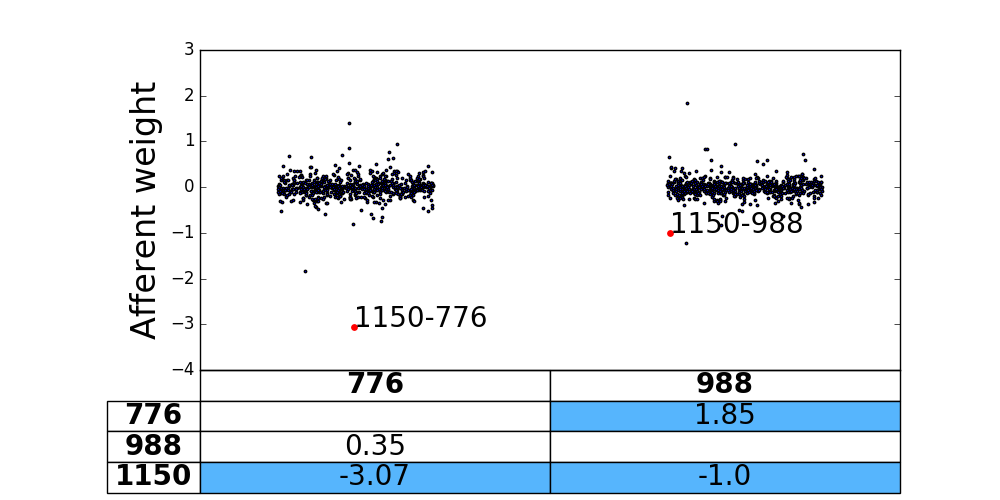
\includegraphics[height=3.5cm,width=\textwidth]{Figures/gate_Input_afferent_interactions.png}
            \caption{Input gate}
            \label{fig:interaction-input}
    \end{subfigure}
    \begin{subfigure}{0.49\textwidth}
           \centering
          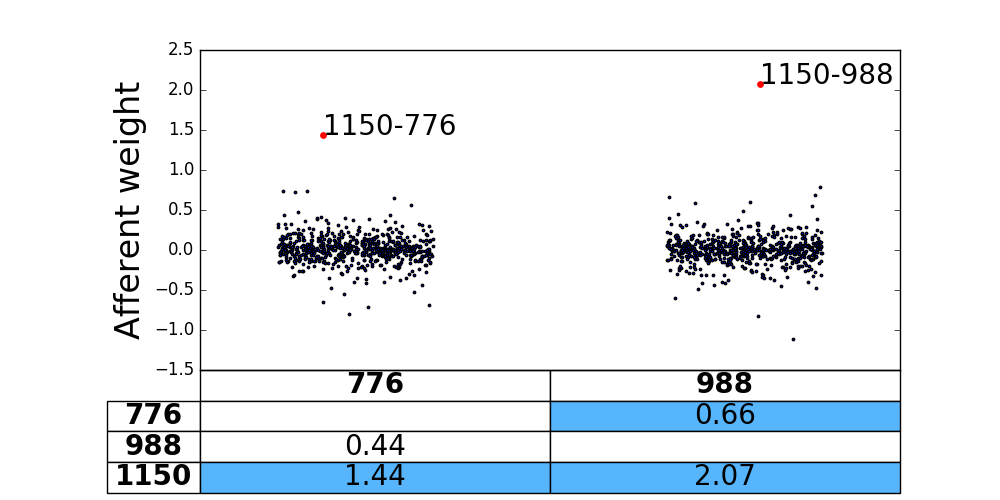
\includegraphics[height=3.5cm,width=\textwidth]{Figures/gate_Forget_afferent_interactions.png}
          \caption{Forget gate}
          \label{fig:interaction-forget}
    \end{subfigure}
    \caption{Connectivity among the syntax unit \unit{2}{500} and
      LR-number units \unit{2}{126} and \unit{2}{338}. Projecting
      units are on the table rows. Blue background highlights outlier
      values ($|z-score|>3$). Weights from the syntax unit are marked in red
      and are explicitly labeled in the plots, which show the overall distributions of afferent weights to each number unit.}
\label{fig:interaction}
\end{figure*}

We finally look at the connections that were learned by the LSTM
between syntax unit \unit{2}{500}, which appears to be more closely involved in
tracking subject-verb agreement, and the LR number units, as well as at
the connections between the latter. For each unit pair, there are 4
connection types, one for each component of the target cell (to the 3
gates and to the update candidate). We focus on input and forget gates, as they control the flow and storage of number information.

Figures \ref{fig:interaction-input} and \ref{fig:interaction-forget}
show the distributions of all afferent recurrent weights to the input
and forget gates of the LR-number units, scaled by the maximal activity
$h_t$ of the pre-synaptic units during the nounPP task (this scaling evaluates
the \textit{effective} input to the units, and did not change the conclusions described below). We found that the weights from the
syntax unit to the forget gate of both \unit{2}{126} and \unit{2}{338}
are exceptionally high in the positive direction compared to all other
afferent connections in the network ($z-score=8.1, 11.2$, respectively), and
those to their input gates exceptionally negative ($z-score=-16.2,
-7.2$). Since the cell activity of syntax unit \unit{2}{500} is
positive across the entire subject-verb dependency (e.g., Figure
\ref{fig:syntax-unit-double-subjrel}), the connectivity from the
syntax unit drives the number unit forget gates towards one
($W^f_{776, 1150}h^{1150}>>0$ and $W^f_{988, 1150}h^{1150}>>0$; $t_{subject}<t<t_{verb}$) and their input gates towards zero
($W^i_{776, 1150}h^{1150}<<0$ and $W^i_{988, 1150}h^{1150}<<0$). Looking at the right-hand-side of
Eq.~(\ref{eq:update-rule}), this means that the first term becomes
dominant and the second vanishes, suggesting that, across the entire
dependency, the syntax unit conveys a `remember flag' to the number
units. Similarly, when the activity of the syntax unit becomes
negative at the end of the dependency, it conveys an `update flag'.

Last, we note that the reciprocal connectivity between the two
LR-number units is always positive, to both input and forget
gates (with $|z-score|>3$ for the \unit{2}{126}-to-\unit{2}{338} direction). Since
their activity is negative throughout the subject-verb dependency
(Figures \ref{fig:singular-unit} and \ref{fig:plural-unit}), this means
that they are \textit{mutually inhibiting}, thus steering towards an
unequivocal signal about the grammatical number of the subject to the
output layer.

